
%(BEGIN_QUESTION)
% Copyright 2009, Tony R. Kuphaldt, released under the Creative Commons Attribution License (v 1.0)
% This means you may do almost anything with this work of mine, so long as you give me proper credit

Read and outline the ``Buoyant-Force Instruments'' and ``Torque Tube'' subsections of the ``Displacement'' section of the ``Continuous Level Measurement'' chapter in your {\it Lessons In Industrial Instrumentation} textbook.  Note the page numbers where important illustrations, photographs, equations, tables, and other relevant details are found.  Prepare to thoughtfully discuss with your instructor and classmates the concepts and examples explored in this reading.

\underbar{file i03952}
%(END_QUESTION)





%(BEGIN_ANSWER)


%(END_ANSWER)





%(BEGIN_NOTES)

As liquid rises around a weighted ``displacer'', a greater buoyant force is experienced which makes the displacer seem to be lighter.  This reduction in apparent weight causes the level instrument to output a greater signal.  Static pressure is irrelevant -- only the liquid's density and the volume displaced (which is proportional to level).  $F_{buoyant} = \gamma V$

\vskip 10pt

The displacer typically hangs inside of a vertical pipe called a ``cage'', connected to the process vessel like a sightglass.  Some displacer-type level instruments are ``cageless'' and hang their displacers directly inside the vessel.

\vskip 10pt

Dry calibration is where we intentionally impart an upward force on the displacer while it's hanging in air, to simulate the buoyant force that the liquid normally exerts on it.

\vskip 10pt

Wet calibration is where we intentionally flood the cage in order to simulate a 100\% full condition.

\vskip 10pt

{\it Torque tubes} are commonly used to support the displacer and to transfer the motion to an external mechanism while sealing off pressure from leaking into that mechanism.  They are hollow spring-steel tubes with a blind end, and a rod in the middle transferring motion from the blind end of the tube (where the displacer hangs) to the open end of the tube (where the sensing mechanism is).  As buoyant force changes, the torque tube twists slightly, causing the sensing mechanism to register the motion.





\vskip 20pt \vbox{\hrule \hbox{\strut \vrule{} {\bf Suggestions for Socratic discussion} \vrule} \hrule}

\begin{itemize}
\item{} {\bf In what ways may a buoyancy level instrument be ``fooled'' to report a false level measurement?}
\item{} Describe how a ``wet'' calibration check is performed on a displacer level instrument.
\item{} Describe how a ``dry'' calibration check is performed on a displacer level instrument.
\item{} Explain what each step of the calculation shown in the ``Buoyant-Force Instruments'' subsection of the textbook is for.
\item{} Could the calculation shown in the ``Buoyant-Force Instruments'' subsection of the textbook have been done without converting the liquid density into units of pounds per cubic inch?  If so, describe how.
\item{} What would change about the calibration of a displacer instrument if we replaced the torque tube with one having thinner spring-steel tube walls?
\item{} What would change about the calibration of a displacer instrument if we replaced the torque tube with one having thicker spring-steel tube walls?
\item{} What would change about the calibration of a displacer instrument if we replaced the displacer with one of a wider diameter?
\item{} What would change about the calibration of a displacer instrument if we replaced the displacer with one of a skinnier diameter?
\item{} What would change about the calibration of a displacer instrument if we added more weight to the displacer without changing its external dimensions?
\item{} What would change about the calibration of a displacer instrument if we subtracted weight from the displacer without changing its external dimensions?
\item{} Explain how the Fisher Level-Trol pneumatic sensing mechanism works.  Is it force-balance or motion-balance?
\item{} Identify a practical level-measurement process that would be unsuitable for a displacer-type level instrument, as well as an alternative level-sensing technology that would work better.  
\item{} Are hydrostatic pressure-based level instruments immune from the problems facing displacer-based level instruments?  Explain why or why not.
\end{itemize}







\vfil \eject

\noindent
{\bf Prep Quiz:}

Suppose the liquid level inside the vessel and cage remains constant, but its density happens to increase over time.  How will the displacer respond?

$$\includegraphics[width=15.5cm]{i03952x01.eps}$$

\begin{itemize}
\item{} The displacer will fall (slightly) 
\vskip 5pt 
\item{} The displacer will sink to the bottom
\vskip 5pt 
\item{} The displacer will oscillate up and down
\vskip 5pt 
\item{} The displacer will rise (slightly)
\vskip 5pt 
\item{} The displacer will twist on a vertical axis
\end{itemize}

\vfil \eject

\noindent
{\bf Prep Quiz:}

Suppose the liquid level inside the vessel falls several inches while its density remains constant.  How will the displacer respond?

$$\includegraphics[width=15.5cm]{i03952x01.eps}$$

\begin{itemize}
\item{} The displacer will sink to the bottom
\vskip 5pt 
\item{} The displacer will fall as much as the level
\vskip 5pt 
\item{} The displacer will twist on a vertical axis
\vskip 5pt 
\item{} The displacer will fall (slightly) 
\vskip 5pt 
\item{} The displacer will rise (slightly)
\end{itemize}


%INDEX% Reading assignment: Lessons In Industrial Instrumentation, Continuous Level Measurement (displacement)

%(END_NOTES)


